\documentclass{article}
\usepackage[utf8]{inputenc}

\usepackage[margin=1in]{geometry}
\usepackage{hyperref}
\usepackage{graphicx}
\usepackage{ulem}

\usepackage{titlesec}
\setcounter{secnumdepth}{4}
\setcounter{tocdepth}{4}
\titleformat{\paragraph}
{\normalfont\normalsize\bfseries}{\theparagraph}{1em}{}
\titlespacing*{\paragraph}
%{0pt}{3.25ex plus 1ex minus .2ex}{1.5ex plus .2ex}
{0pt}{1.0ex plus 1ex minus .2ex}{0.1ex plus .2ex}

\newcommand{\name}{ECW\ }
\newcommand{\nameNospace}{ECW}
\newcommand{\namep}{ECW.}

\renewcommand{\labelenumii}{\theenumii}
\renewcommand{\theenumii}{\theenumi.\arabic{enumii}}
\renewcommand{\theenumiii}{\theenumii.\arabic{enumiii}}

\usepackage{fancyhdr}
\pagestyle{fancy}

\lhead{ Responsible: Alexander Ekman, Linnea Johnsson, and David Ravanelli \\ Date: \today}  \rhead{Document number: PUSS21418 \\ Version: 1.8}
\renewcommand{\headrulewidth}{0.5pt} 

\title{SSD - System Specification Document}
\author{Team 1}

\begin{document}

\date{}
\maketitle
\thispagestyle{fancy}
\newpage

\section*{Revision History}
\begin{table}[h]
    \centering
    \begin{tabular}{|l|l|p{55mm}|p{35mm}|}
    \hline
    Date & Version & Description & Author \\ 
    \hline\hline 
    2021-10-13 & 1.0 & Outlines of all sections & Linnea Johnsson \\
    \hline
    2021-10-15 & 1.1 & Added system setup instructions & Alexander Ekman \& Max Fogwall  \\
    \hline
    2021-10-18 & 1.2 & Added all unfulfilled requirements & Alexander Ekman \\
    \hline
    2021-10-19 & 1.3 & Filled in section 1 and 2 & Linnea Johnsson \\
    \hline
    2021-10-20 & 1.4 & Added unfulfilled requirements left after the internal deadline & Alexander Ekman \\
    \hline
    2021-10-20 & 1.5 & Updated install instructions & Alexander Ekman \\
    \hline
    2021-10-20 & 1.6 & Added user instructions for all system features, including figures & Alexander Ekman \\
    \hline
    2021-10-20 & 1.7 & Updated completed issues, added matched cases in routes figure, and updated figure captions & Alexander Ekman \\
    \hline
    2021-10-20 & 1.8 & Proofreading & Alexander Ekman \\
    \hline
    \end{tabular}
    \label{tab:history}
\end{table}
\newpage

\begin{thebibliography}{widest entry}

    \bibitem{PH} "Programvaruutveckling för Stora System Projekthandledning 2021", Chapter 9, Institutionen för Datavetenskap Lunds Tekniska Högskola, Lunds Universitet, 26 August 2021
    
    \bibitem{SDP} "SDP - Software Development Plan, Team 1 - ETSN05", Alexander Ekman and Linnea Johnsson, url=\url{https://github.com/exook/ETSN05_team1_documents/blob/main/SDP.tex}, accessed \today
    
    \bibitem{PRD} "PRD - Product Requirements Document, Team 1", Alexander Ekman and Linnea Johnsson, url=\url{https://github.com/exook/ETSN05_team1_documents/blob/main/PRD.tex}, accessed \today
    
\end{thebibliography}
\newpage

\tableofcontents
\newpage

%Från projekthandledningen:
%I SSD ska systemets olika dokument “knytas samman” till ett system. SSD ska innehålla en beskrivning av det levererade systemets olika delar, versioner etc. 
%SSD ska även innehålla en beskrivning av eventuella skillnader gentemot PDR. Alla större förändringar av PDR eller förändringar av PDR som har betydelse för kunden skall beskrivas. 
%Om några krav inte kunnat uppfyllas skall detta tydligt anges med hänvisning till relevanta testfall och testprotokoll. 
%Det är mycket viktigt att det i SSD står var man kan hitta alla dokument och filer, samt hur man startar systemet.

\section{Introduction}\label{sec:intro} %Linnea
%This document presents describes the delivered system, and details which version each document is in.  It also specifies limitations of the delivered system, and possible differences between the requirements specification and the delivered system.
This document aims to present and describe the carpool web-app delivered as part of the course ETSN05. The documents, and which versions of them, that are related to the system are listed. Furthermore, this document describes the system's limitations. The limitations are presented as the differences between the final delivered system and the system described in the Product Requirements Document (PRD) \cite{PRD}. Lastly, this document provides instructions on how to set up the system and use the web-app.

\section{Delivered system} %Linnea
%The delivered system consists of the following documents/parts: *tabell över dokumenten*

%Software Product Features Backlog(SPF) - PUSS21413
%Sprint log/plan (SP) - PUSS21414

The system consists of the code based product as well as multiple documents that corresponds to the system in different ways. In table \ref{tab:deliveredSys} these documents, and how they relate to the delivered system, is presented. 

\begin{table}[h]
    \centering
    \begin{tabular}{|l|l|l|p{90mm}|}
    \hline
    Document & Document number & Version & Purpose in the system \\
    \hline \hline
    %SDP & PUSS21411 & 1.3 & \\ \hline
    PRD & PUSS21412 & 1.21 & Contains the requirements of the system, and more. \\ \hline
    STLDD & PUSS21415 & 1.29 & The high level design of the system \\ \hline 
    SDD & N/A & N/A & The actual code base and its corresponding comments \\ \hline
    SVVR & PUSS21417 & 1.11 & Comparisons of the code and the user stories from the PRD. Contains unit tests, integration tests and review protocols. \\ \hline
    SSD & PUSS21418 & 1.8 & A description of the delivered system and how it differs from the ordered one \\ \hline
   % PFR & PUSS21419 & TODO & \\ \hline
    \end{tabular}
    \caption{The documents, and their current version, related to the delivered system.}
    \label{tab:deliveredSys}
\end{table}


\section{Limitations}
%ingen text från exemplet?

\subsection{System objective} %Alexander
%The intention is that the delivered system should be used as a base for further development of web-based systems.  It is not meaningful to deliver the system to a real user as it is today, as the only functionality it includes is a possibility to login and logout.  This means that the system has not been tested in practice with real users.

The objective of the delivered system is that it should be used as a base for further development. There is no intention to deliver the system to real users in its current state. This is because some functionality is not yet finalized, and the system has not been tested in practice with real users.

\subsection{Differences compared to the PRD} %Alexander
\subsubsection{Maven support}
The PRD did not specify a requirement for Maven. However, Maven is recommended for running the system.

\subsubsection{Functional requirement F2: Driver registration}
"A prospective user registering as a driver, or a rider and a driver must also register car brand, model, color, and licence plate number"\cite{PRD}. In the delivered version, drivers can register a car, however this is done in the route submission window seen in Figure \ref{fig:create_route}. When a user selects "driver" on the submissions page, they are asked to add a vehicle to the submission. If they haven't registered a car before, they have the option to add a new car as seen in Figure \ref{fig:add_vehicle}. Once a car is added they can select it from a drop-down menu in any future submissions.

\subsubsection{Functional requirement F8: Profile Details}\label{profile_details}
"A logged in user should be able to see and edit some of their profile details"\cite{PRD}. The delivered system will not support users editing the profile details or a profile page. If a user needs something changed they must contact someone with admin and they would perform the appropriate change.

\subsubsection{Functional requirement F10: Necessary contact details}
"A logged in user who is matched with a rider/driver should see the upcoming routes and
details of that route on their profile page"\cite{PRD}. In the delivered system, this information is instead shown under "Your routes" as shown in Figure \ref{fig:your_routes}.
%Further more, there was not enough time to implement the sharing of contact details for matched users. This should however be a priority in any future work.

\subsubsection{Functional requirement F11: Upcoming travel}
"A logged in user who is matched with a rider/driver needs to accept or decline matches with riders/drivers"\cite{PRD}. The delivered system does not support users accepting or declining matches. If there is a change of plans, the two users will have to contact each other instead.

\subsubsection{Functional requirement F12: Match notification}
"When a user is matched with a driver/rider they should be notified in the web app"\cite{PRD}. The delivered system does not notify users once a match is achieved between a rider and a driver. Instead users will have to check their "Your routes" page for updates on their upcoming routes and matched routes, as shown in Figure \ref{fig:your_routes}.

%\subsubsection{Functional requirement F13: Admin log in}
%"As administrator of the system I should be able to log in and obtain extra privileges as administrator."\cite{PRD}. The administrator is able to log in and remove users as stated in the requirements. However, since it was not a requirement, the admin was never given the functionality to edit other user profile details. With the delivered version of the system not being able to allow users to edit their own profile details, it is important to note that neither the administrator nor a users can edit profile details. Should a user need their details changed, they would have to contact an admin and have their old profile removed and replaced with a new profile.

\subsubsection{Performance Requirement Per1: Entering correct username and password}
"A user who enters a correct username and password, once pressing the ”log in” button, should not wait longer than 2 seconds to see the submission page"\cite{PRD}. A user entering the correct username and password is logged in within 2 seconds, however, they are not directed to the submissions page as the main page. In the delivered system, the main page is a neutral page which offers the logged in user with a choice to select either "Create Route", "Your routes" as seen in Figure \ref{fig:main_page}. This layout does not affect the core functionality of the system, but it does deviate from the user interface prototypes in Figure 4, 5 , 6, and 7, and some of the wording of the PRD\cite{PRD}.

\subsubsection{Performance Requirement Per2: Entering incorrect username and password}
"A user who enters an incorrect username and password, once pressing the ”log in” button, should not wait longer than 2 seconds to be prompted for another attempt"\cite{PRD}. If the username and password are incorrect the user is allowed to attempt again within 2 seconds. Providing a proper error message has not been a priority, and is not implemented in the delivered system.

\subsubsection{Performance Requirement Per3: Notification of new match}
"After a driver/rider is matched, their profile pages should update accordingly within 10 seconds"\cite{PRD}. As specified in Section \ref{profile_details}, the delivered version does not include a profile page. However, the match is displayed on the "Your routes" page within 10 seconds.

\subsubsection{Reliability Requirement R1: User input}
"The web-app should not crash or freeze due to user input"\cite{PRD}. With a small team there was not enough time to do the large scale testing which would guarantee that no user input would crash the system. However, no user input should crash the server, but it could perhaps freeze the users browser session.

\subsubsection{Usability Requirement U3: User browser and operating system}
"The system should work the same for users using Microsoft Edge, Google Chrome, Mozilla Firefox, or Safari web browsers. It should also be independent from their operating system"\cite{PRD}. The delivered system does not perform well on Firefox due to some issues with sending POST-requests. Chromium based browsers and Safari are known to work.

\subsubsection{Portability Requirement Por1: Remote/local host}
"The system should be able to run in full on a local or remote host"\cite{PRD}. The delivered system has only been tested running on a local host. Since this is impractical for any commercial use, making it run on a remote host should be a top priority in the future.

\subsubsection{Usability Requirement U2: Multiple users}
"Multiple users should be able to be logged in and use the system features in parallel"\cite{PRD}. As the delivered system has not been tested on a remote host, having users acting in parallel has also not been fully tested. However, it seems to work on a local host.

\subsubsection{Usability Requirement U4: Mobile support}
"Users should be able to use the web-app from their mobile devices without suffering from decreased usability compared to using a PC"\cite{PRD}. As the delivered system has not been tested on a remote host, it has been impossible to test the mobile support.

\section{Installation instructions} %Alexander
\subsection{Setup instructions: Eclipse}
\subsubsection{Initial setup}
\begin{itemize}
\item Download and install Eclipse from \url{https://www.eclipse.org/}
\item Clone the repository: using "git clone \url{https://coursegit.cs.lth.se/alma.orucevic-alagic/} \\ 
\url{etsn05-team1.git}"
\item Start Eclipse (Version 4.21.0 or newer)
\item Select the cloned repository as the workspace, press "Launch"
\item Exit the Eclipse welcome window if there is any
\item Go to file \url{->} Import
\item Select "Maven" and then "Existing Maven Projects", Press "Next"
\item In the "Import Maven Project" window, select the root directory as "\url{etsn05-team1/base/server}"
\item Back at the "Import Maven Project" window, click the "Add project(s) to working set" box
\item Click "Finish"
\end{itemize}

\subsubsection{Starting the server}
\begin{itemize}
\item Make sure you are in the correct workspace
\item Navigate to \url{"etsn05-team1/base/server/src/main/java/se.lth.base.server"}
\item Select and run "BaseServer.java". On the first execution, this also sets up the database.
\item If there are remnants left from a previous system setup (Old routes, profiles etc), navigate to \url{"etsn05-team1/base/server/src/main/java/se.lth.base.server.database"} and run "CreateSchema.java"
\end{itemize}


\subsection{Setup instructions:  Visual Studio Code}

\subsubsection{Initial and starting the server}
\begin{itemize}
\item Download and install Visual Studio Code (\url{https://code.visualstudio.com/})
\item Clone the repository: "git clone \url{https://coursegit.cs.lth.se/alma.orucevic-alagic/} \\
\url{etsn05-team1.git}"
\item Open the cloned repository with Visual Studio Code
\item Navigate to "\url{etsn05-team1/base/server/src/main/java/se/lth/base/server}"
\item Select and run "BaseServer.java"
\item Go to Run and Debug in the left-hand menu bar
\item Click on Run and Debug. On the first execution, this also sets up the database.
\item If there are remnants left from a previous system setup (Old routes, profiles etc), navigate to \url{"etsn05-team1/base/server/src/main/java/se.lth.base.server.database"} and run "CreateSchema.java"
\end{itemize}


\subsection{Logging in and registering new user}
Once the server is started you can go to \url{http://localhost:8080/login/login.html} and log in using one of the pre-existing credentials found in Table \ref{passwords}. To register a new user, go to \url{(http://localhost:8080/register/register.html}

\begin{table}[h!]\label{passwords}
    \centering
    \begin{tabular}{|c|c|c|}
        \hline
         Username & Password & Role \\\hline\hline
         Admin & password & ADMIN \\\hline
         Test & password & DRIVER \\\hline
         Passenger & password & PASSENGER \\\hline
        Driver & password & DRIVER \\\hline
        Both & password & BOTH\\\hline
    \end{tabular}
    \caption{The available credentials after the first time setup of the system}
    \label{tab:my_label}
\end{table}

\clearpage
\newpage
\section{User instructions}
\subsection{Log in screen}
The log in screen when the local host server is running can be found at \url{http://localhost:8080/login/login.html}. Here, the user or admin is promted to log in or register, as shown in Figure \ref{fig:login_register}

\begin{figure}[h!]
    \centering
    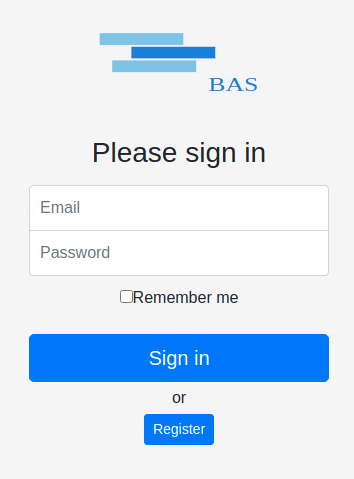
\includegraphics[scale=0.5]{ssdFigures/login_register.png}
    \caption{The log in page}
    \label{fig:login_register}
\end{figure}

\clearpage
\newpage
\subsection{User registration}
By clicking the "Register" button seen in Figure \ref{fig:login_register}, the user is taken to the registration screen shown in Figure \ref{fig:register}. The user here selects a "role", i.e. if they will be a driver, passenger, or both. Choosing "both" will give them the most flexibility later on. Once all the fields are filled in, they click "Register me".

\begin{figure}[h!]
    \centering
    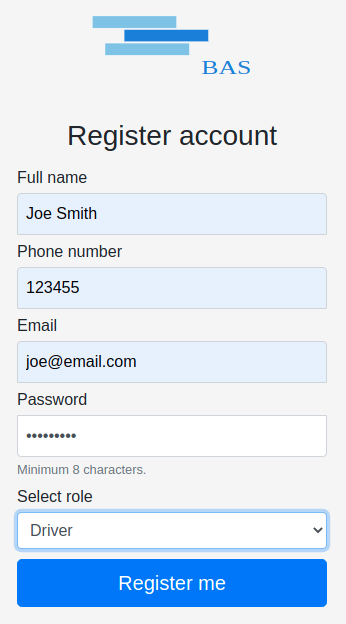
\includegraphics[scale=0.5]{ssdFigures/register.png}
    \caption{The user registration page}
    \label{fig:register}
\end{figure}

\clearpage
\newpage
\subsection{Main page}
Once a registered user logs in they are taken to the main page, seen in Figure \ref{fig:main_page}. By clicking "Create Route" they are taken to the "Create Route Page", where drivers can submit that they are driving somewhere, and passengers can submit that they would like to carpool somewhere. By clicking "Your routes" the user will be taken to the "Your routes page", here they can see information of upcoming travel, and matches with other drivers/passengers. At the top of the main page the users can navigate between the pages and sign out.

\begin{figure}[h!]
    \centering
    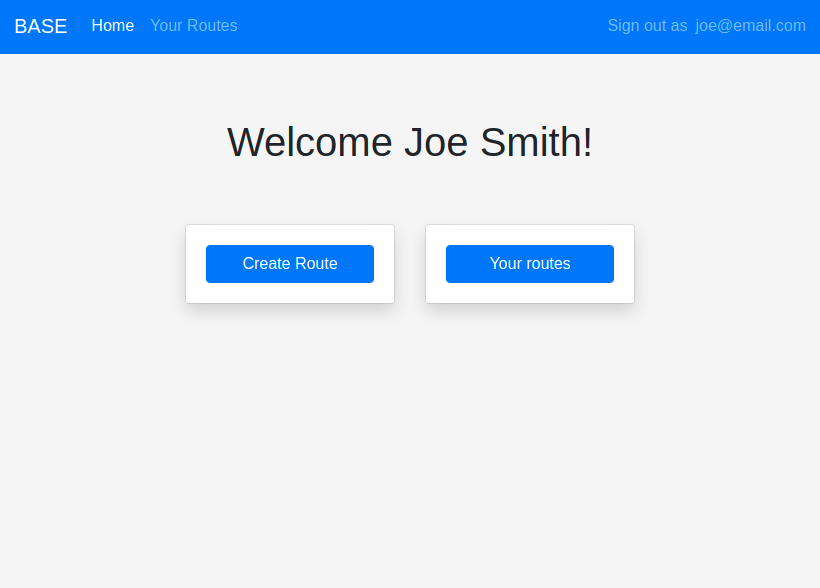
\includegraphics[scale=0.5]{ssdFigures/main_page.png}
    \caption{The main page}
    \label{fig:main_page}
\end{figure}

\clearpage
\newpage
\subsection{Create Route Page}
The "Create Route Page" is where drivers can submit that they are driving somewhere, and passengers can submit that they would like to carpool somewhere. This page looks different for drivers and passengers. Both user roles submit a Start, End, Departure, and Arrival. But only the driver adds a vehicle and the number of available seats. To add a vehicle from the drop-down menu, the driver first needs to click "Add Vehicle", if this hasn't been done before for that user. When the user clicks "Create route", their route is registered in the database and matched to any users with similar routes.

\begin{figure}[h!]
    \centering
    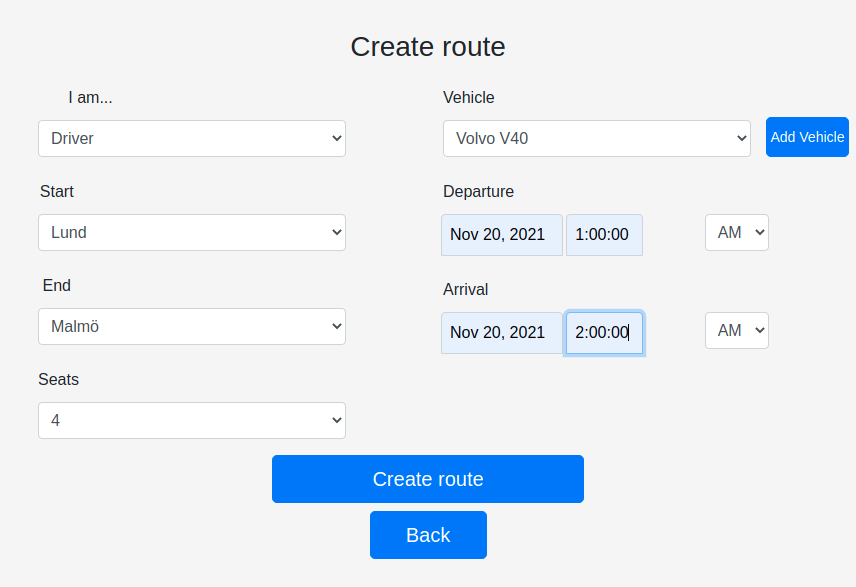
\includegraphics[scale=0.48]{ssdFigures/create_route.png}
    \caption{The "Create Route Page"}
    \label{fig:create_route}
\end{figure}

\clearpage
\newpage
\subsection{Add Vehicle}
When a driver clicks on the "Add Vehicle" button in the "Create route page" they are taken to the "Add Vehicle page". Here drivers enter details regarding their vehicle as shown in Figure \ref{fig:add_vehicle}. These details will be crucial for passengers to identify the driver when being picked up.

\begin{figure}[h!]
    \centering
    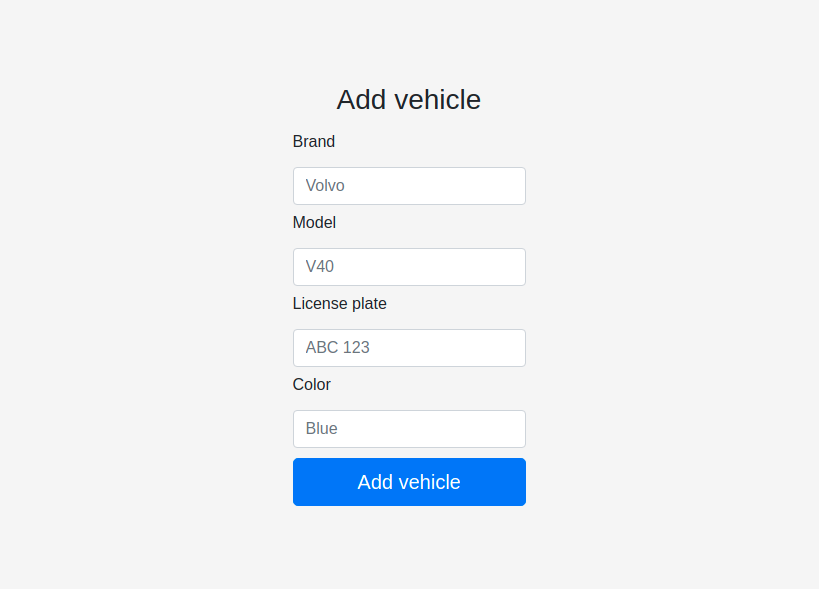
\includegraphics[scale=0.5]{ssdFigures/add_vehicle.png}
    \caption{The "Add Vehicle Page"}
    \label{fig:add_vehicle}
\end{figure}

\clearpage
\newpage
\subsection{Your Routes page}
By clicking "Your Routes" from the main page, a user can see the routes that they have submitted, as well as routes which have been matched with other drivers/passengers. This is shown in Figure \ref{fig:your_routes}.

\begin{figure}[h!]
    \centering
    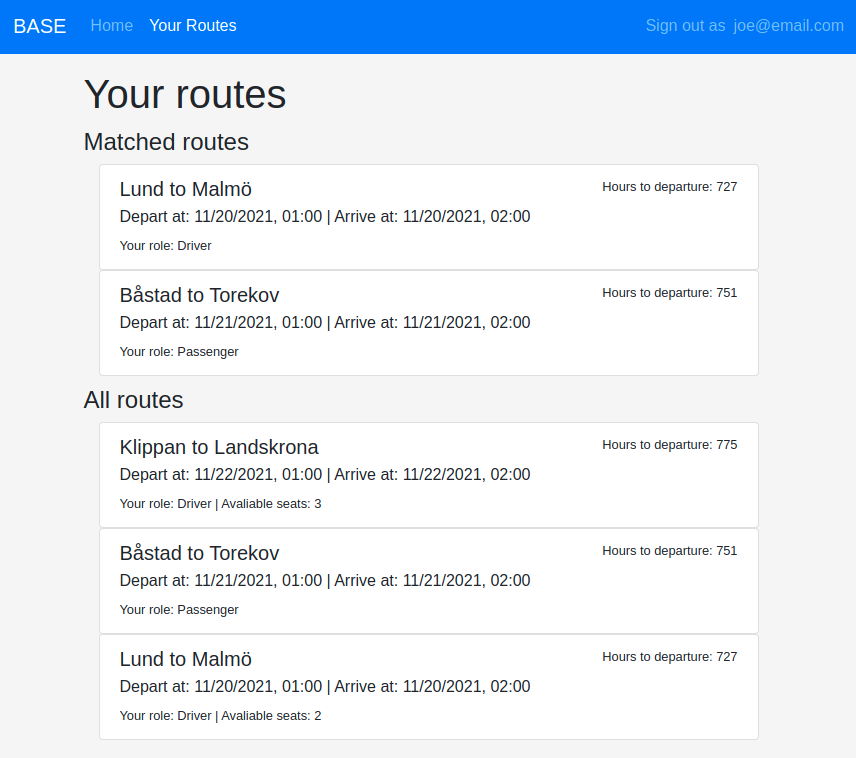
\includegraphics[scale=0.5]{ssdFigures/your_routes.png}
    \caption{The "Your Routes Page" }
    \label{fig:your_routes}
\end{figure}

\clearpage
\newpage
\subsection{Admin Main Page}
Logging in as admin shows a very similar page as a regular user. However, in the top navigation bar there is the added "User Admin" tab as seen in Figure \ref{fig:admin_main_page}.

\begin{figure}[h!]
    \centering
    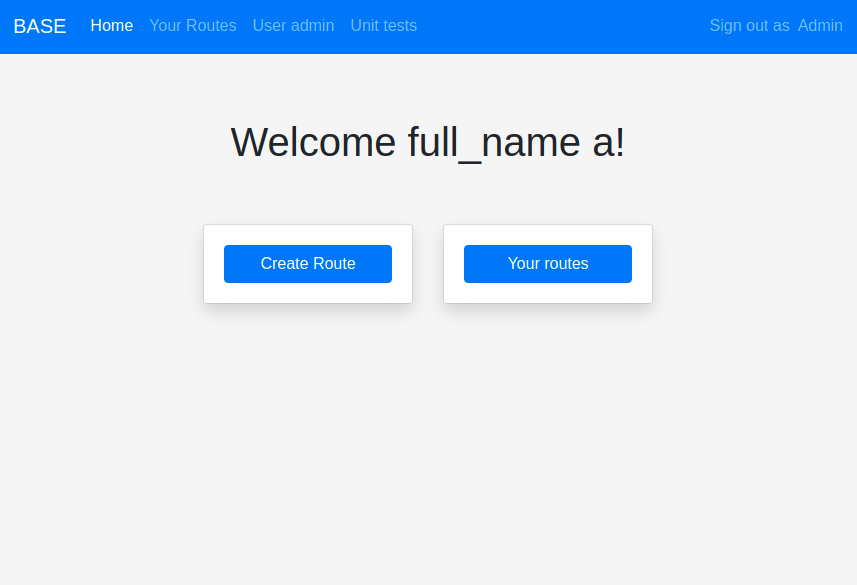
\includegraphics[scale=0.5]{ssdFigures/admin_main_page.png}
    \caption{The admin main page, which has the addition to navigate to the "User admin" page}
    \label{fig:admin_main_page}
\end{figure}

\clearpage
\newpage
\subsection{Admin Changing User Profiles}
As seen in Figure \ref{fig:admin_profile_details}, an admin in the "User Admin page" can add or remove users. They can also change the profile details of users. This is a very important admin feature since the delivered system does not allow users to edit this themselves.

\begin{figure}[h!]
    \centering
    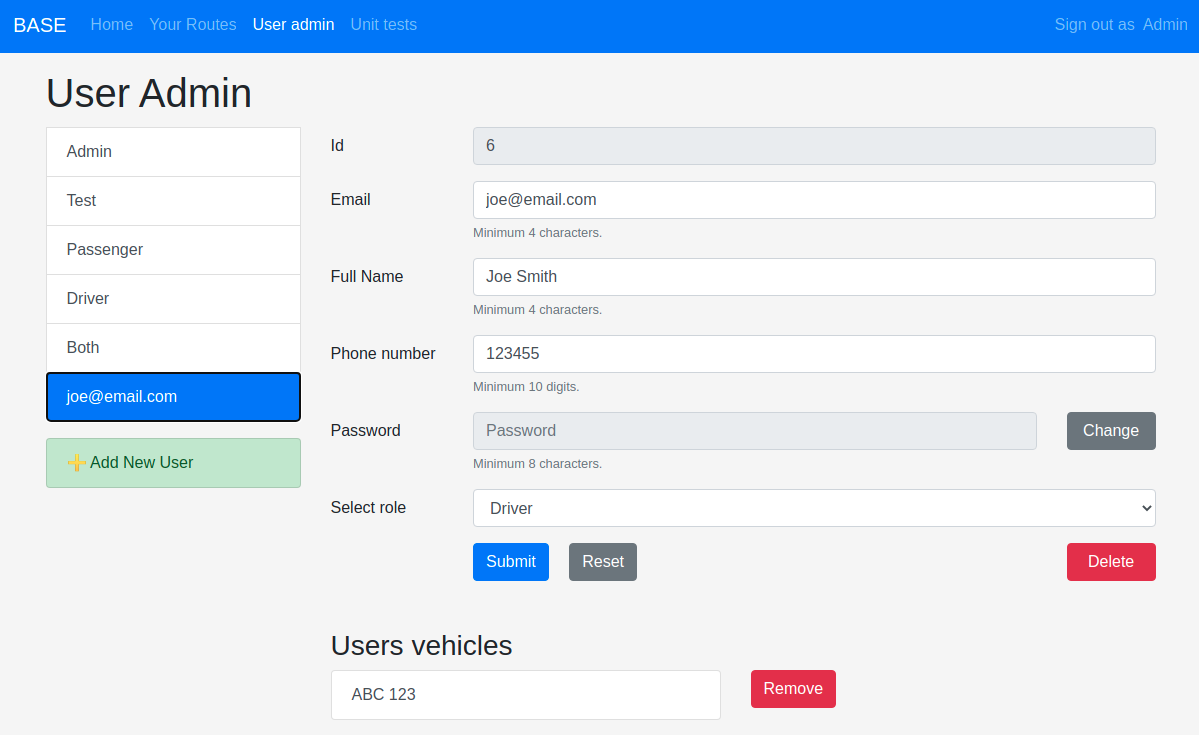
\includegraphics[scale=0.40]{ssdFigures/admin_profile_details.png}
    \caption{The user admin page where the admin can change profile details}
    \label{fig:admin_profile_details}
\end{figure}

\end{document}